\section{Configuration Tab}
\label{sec:osgview_config}

\begin{figure}[H]
    \hspace*{-2cm}
    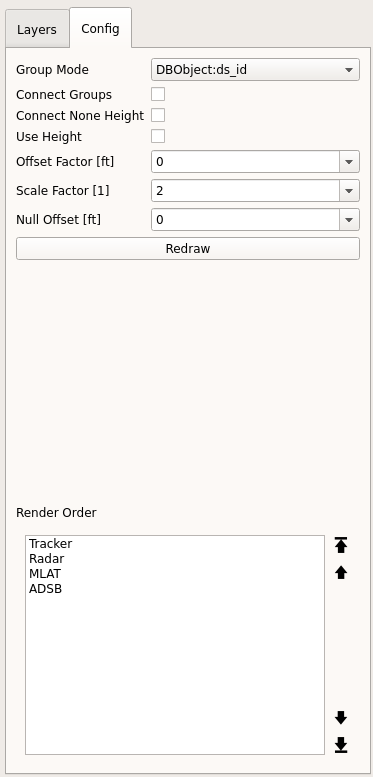
\includegraphics[width=8cm,frame]{../screenshots/osgview_config_tab.png}
  \caption{OSG View Config tab}
\end{figure}


In the 'Config' tab, several elements exist:

\begin{itemize}
 \item Group Mode: Defines how layers are generated. Refer to Section \ref{sec:group_mode} for details.
 \item Connect Groups: Whether grouped target reports should be connected using lines
 \item Connect None Height: If groups are connected, whether target reports with not height information should be connected
 \item Use Height: Whether height information should be used to create a 3D presentation
 \item Offset Factor: If height information is used, this factor is added to the height
 \item Scale Factor: If height information is used, this factor is used to multiply the height
 \item Null Offset: If height information is used, this factor is used for target reports without height information
 \item Redraw button: Triggers a re-draw of the geometry, e.g. after a one of the above options was used
 \item Render Order: Defines the drawing order of DBObjects. To bottom one is drawn first, the top one last (over all others)
\end{itemize} 

\subsection{Group Mode}
\label{sec:group_mode}

In this selection the way layers are generated can be changed. \\\\

The following items can be present in the list:

\begin{itemize}
 \item DBObject: DBObject type, e.g. Radar, MLAT, ...
 \item ds\_id: Data source identifier, e.g Radar1, Radar2, ARTAS
 \item target\_addr: Mode S Address
 \item track\_num: Track number (local or system)
 \item mode3a\_code: Mode 3/A code
 \item UTN: Unique Target Number, only available if association information is present
\end{itemize}
\ \\

The group mode defines what layers are generated, e.g. for 'A' only layers for all values of 'A' are created, for 'A:B' layers for all values of 'A' are created, each with sub-layers for all values of 'B'. In this case, 'A' is the parent, 'B' is the child. \\\\

If no values exist in the data for a layer, this data is grouped in the layer 'None'.\\\\

The following modes exist: \\

\begin{itemize}
 \item DBObject
 \item DBObject:ds\_id
 \item DBObject:ds\_id:target\_addr
 \item DBObject:ds\_id:track\_num
 \item DBObject:ds\_id:mode3a\_code
 \item UTN:DBObject
 \item UTN:DBObject:ds\_id
 \item UTN:DBObject:ds\_id:target\_addr
 \item UTN:DBObject:ds\_id:track\_num
 \item UTN:DBObject:ds\_id:mode3a\_code
 \item mode3a\_code:DBObject
 \item mode3a\_code:DBObject:ds\_id
 \item target\_addr:DBObject
 \item target\_addr:DBObject:ds\_id
\end{itemize}
\  \\

Please note that the UTN group modes only exist when association information is present.

\paragraph{DBObject:ds\_id}

In this group mode the DBObject name is used to create the first layer, with sub-layers for each data source.

\begin{figure}[H]
    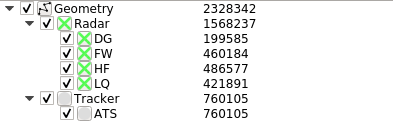
\includegraphics[width=10cm,frame]{../screenshots/osgview_group_dbo_ds.png}
  \caption{OSG View group mode DBObject:ds\_id}
\end{figure}

\paragraph{mode3a\_code:DBObject}

In this group mode the Mode 3/A code is used to create the first layer, with sub-layers for each DBObject.

\begin{figure}[H]
    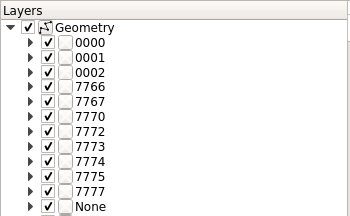
\includegraphics[width=10cm,frame]{../screenshots/osgview_group_ma_dbo.png}
  \caption{OSG View group mode mode3a\_code:DBObject}
\end{figure}

\paragraph{DBObject:ds\_id}

In this group mode the DBObject name is used to create the first layer, with sub-layers for each data source.

\begin{figure}[H]
    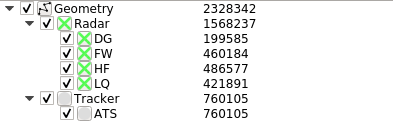
\includegraphics[width=10cm,frame]{../screenshots/osgview_group_dbo_ds.png}
  \caption{OSG View group mode DBObject:ds\_id}
\end{figure}

\paragraph{mode3a\_code:DBObject}

In this group mode the Mode 3/A code is used to create the first layer, with sub-layers for each DBObject. All target reports without a Mode 3/A code are grouped into layer 'None'.

\begin{figure}[H]
    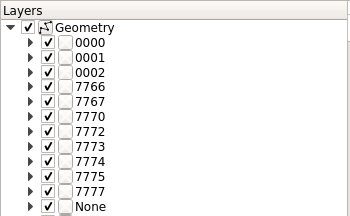
\includegraphics[width=10cm,frame]{../screenshots/osgview_group_ma_dbo.png}
  \caption{OSG View group mode mode3a\_code:DBObject}
\end{figure}

\paragraph{UTN:DBObject}

In this group mode the UTN is used to create the first layer, with sub-layers for each DBObject. All target reports without a UTN (not used by ARTAS) are grouped into layer 'None'.  \\

Currently the sorting is alphanumeric, so the ordering is not perfect. This will be improved in the future.

\begin{figure}[H]
    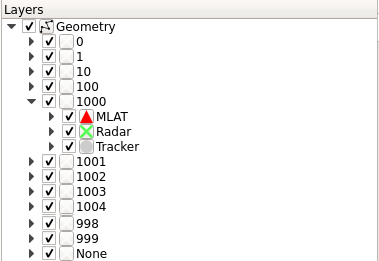
\includegraphics[width=10cm,frame]{../screenshots/osgview_group_utn_dbo.png}
  \caption{OSG View group UTN:DBObject}
\end{figure}

\subsubsection{Group Lines}

Group lines are current drawn for all target reports in the last group in the layers. If the 'Connect Groups' checkbox is set, connection lines between all target reports in the same group are drawn, except for the 'None' group.

\begin{figure}[H]
    \hspace*{-2cm}
    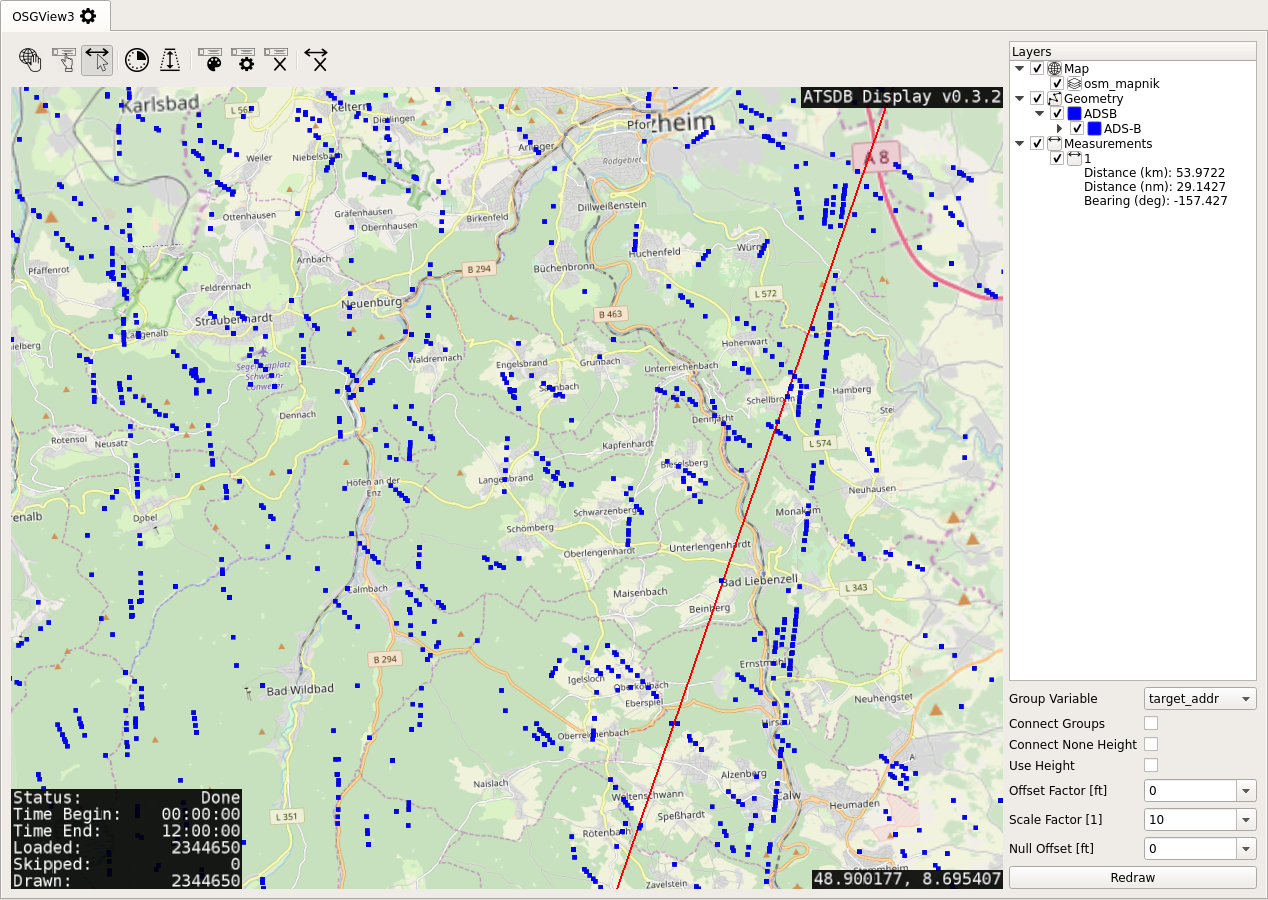
\includegraphics[width=18cm,frame]{../screenshots/osgview_no_lines.png}
  \caption{OSG View Data without lines}
\end{figure}

If the height information is used (3D view), if target reports without height information are connected, the lines clutter the display. The 'Connect None Height' checkbox allows to set the behaviour. \\

Please \textbf{note} that changes both these values requires a manual redraw using the 'Redraw' button.

\subsection{Height Operations}

Per default, a target reports height is not used for display, which is common in current air-traffic displays. However, in certain situation a true 3D display might be of interest to a user, and therefore several options where incorporated:

\begin{itemize}
 \item Use Height: Use the height based on Mode C $h_c$, transformed to meters
 \item Offset Factor: If height information is used, this factor $h_o$ is added to the height
 \item Scale Factor: If height information is used, this factor $h_s$ is used to multiply the height
 \item Null Offset: If height information is used, this factor $h_n$ is used for target reports without height information
\end{itemize}

Generally, if no height information is given (no Mode C code), the height is either $0$ or the height offset (if used). That means that those target reports appear to the on the ground. If connection lines are drawn between the ones in the air and those without, a lot of annoying lines are shown.

The formula to calculate the height (if existing) is as follows:

$$ h = h_o + h_s \cdot h_c [m]$$ 

If no height information is given:

$$ h = h_n [m]$$ 

Please note that upon changes to the height usage, a manual redraw has to be performed using the 'Redraw' button.


\begin{figure}[H]
    \hspace*{-2cm}
    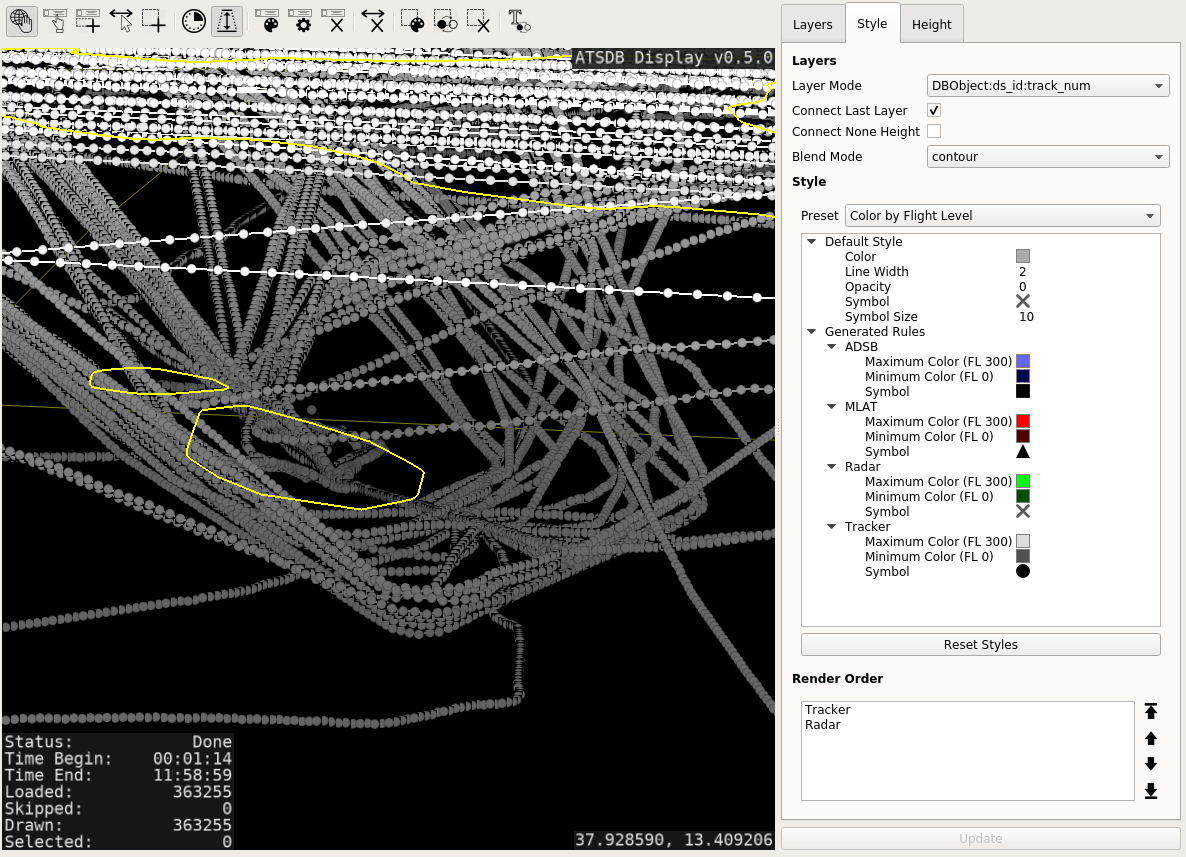
\includegraphics[width=18cm,frame]{../screenshots/osgview_use_height.png}
  \caption{OSG View use height}
\end{figure}

\subsection{Render Order}

In the render order widget, the drawing order of all DBObjects is specified. The one at the top is drawn last (over all others), so it is useful to move the most important DBObject (for the current inspection) to the top.

\begin{figure}[H]
    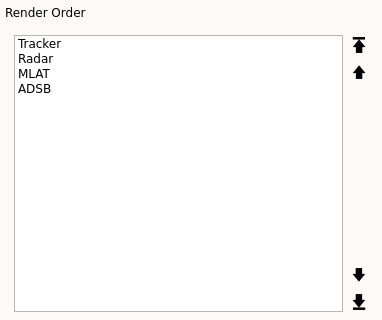
\includegraphics[width=10cm,frame]{../screenshots/osgview_render_order.png}
  \caption{OSG View render order}
\end{figure}

To change the drawing order click on the DBObject to move and use the buttons on the right side. Please note that no redraw is required and that the drawing order is persisted in the configuration.
% 
 \begin{itemize}
 \item 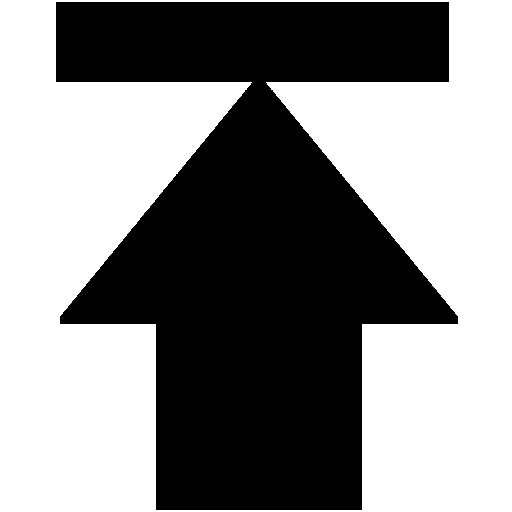
\includegraphics[width=0.5cm]{../../data/icons/top.png} Move to Top: Move DBO to top position
 \item 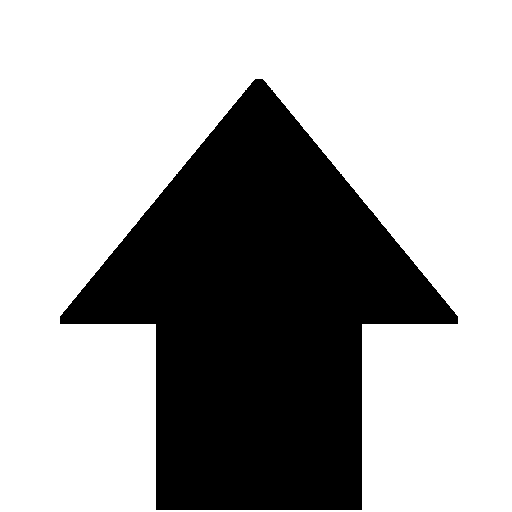
\includegraphics[width=0.5cm]{../../data/icons/up.png} Move Up: Move DBO one position up
 \item 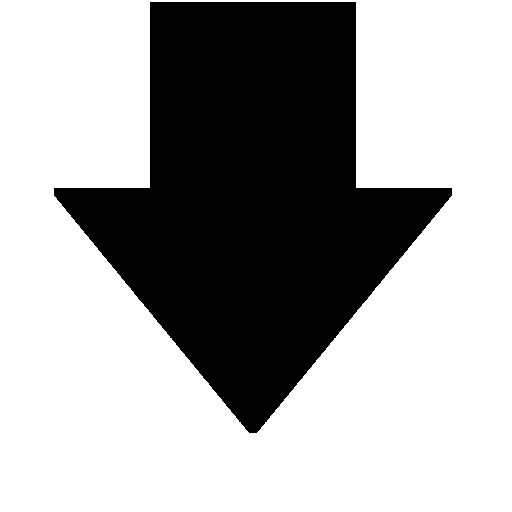
\includegraphics[width=0.5cm]{../../data/icons/down.png} Move Down: Move DBO one position down
 \item 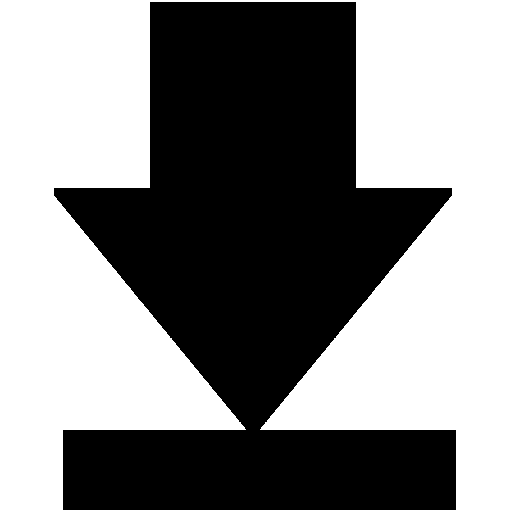
\includegraphics[width=0.5cm]{../../data/icons/bottom.png} Move to Bottom: Move DBO to the bottom position
\end{itemize}
